\section{Langages de programmation}
\label{langages}
Cette partie traite des différents éditeurs et langages de programmation utilisés dans les organisations présentées au point précédent.

\subsection{Blockly}
\label{blockly}

\begin{figure}[!ht]
  \begin{center}
    
\includegraphics[scale=0.5]{content/5-related_work/images/blocky}
    \caption{Logo de Blocky}
    \label{fig:blocky}
  \end{center}
\end{figure}
Blockly \cite{blockly} est un langage de programmation graphique basé sur des technologies du web.

Blockly a comme particularité :
\begin{itemize}
\item de s'exécuter dans un navigateur ;
\item d'exporter du code source en JavaScript, Dart, etc. ;
\item d'être open source ;
\item d'être haut niveau.
\end{itemize}

Il n'est pas directement une plateforme d'éducation dans le sens où il peut être utilisé autant pour l'éducation que pour le business, les jeux \ldots en fonction des \glspl{bloc} implémentés. En effet, Blockly est juste une interface graphique en pièces de puzzle sur des fonctions écrites en JavaScript. Celles-ci permettent d'intéragir avec le domaine d'utilisation. Il faut donc que pour chaque domaine une implémentation soit réalisée.\\

Blockly a été conçu avec certaines propriétés choisies lors de sa création. Les trois premières augmentent la compréhension des néophytes, les autres portent sur des facilités du langage. Les propriétés décidées lors de la conception du langage sont \cite{blockly-lang} :

\begin{itemize}
  \item des indices de listes commençant à 1 ;
  \item des noms de variables non sensibles à la casse ;
  \item pas de portée de variables, elles sont toutes globales ;
  \item la possibilité de faire un export en JavaScript ;
  \item un code natif généré proche de celui des \glspl{bloc}.
\end{itemize}

\subsection{Scratch}

\begin{figure}[!ht]
  \begin{center}
    
\includegraphics[scale=0.4]{content/5-related_work/images/scratch}
    \caption{Logo de Scratch}
    \label{fig:scratch}
  \end{center}
\end{figure}
Scratch \cite{scratch} est un langage de programmation graphique développé par le MIT pour apprendre aux enfants la programmation. C'est l'interface qui permet de faire des \glspl{script} facilement grâce à une programmation par \glspl{bloc} et du glisser-déposer.\\

Il a été pensé pour être un outil créatif pour réaliser des histoires, des jeux, des simulations, de l'art, etc. Il a, par exemple, son propre éditeur d'image et de son. Un autre but de ce langage est d'être simple à utiliser et à apprendre. Il a en effet été conçu pour des enfants n'ayant aucune connaissance préalable en programmation.\\

Actuellement Scratch est à sa version 2 qui est une version web. Cette version a été complètement réécrite en flash par rapport à la version 1 en Smalltalk. De plus, la version 2 n'est plus open source contrairement à la première version.

Comme le montre la figure \ref{fig:scratch-printscreen}, l'interface de Scratch se divise en plusieurs grandes parties :

\begin{enumerate}
\item sur la gauche, il y a la zone de dessin dans laquelle s'anime les composants graphiques des \glspl{script} ;
\item au milieu, une liste des \glspl{bloc} disponibles triés par catégorie ;
\item sur la droite, la zone de \gls{script} qui contient tous les \glspl{script} liés au \gls{sprite} sélectionné.
\end{enumerate}

\begin{figure}
  \begin{center}
    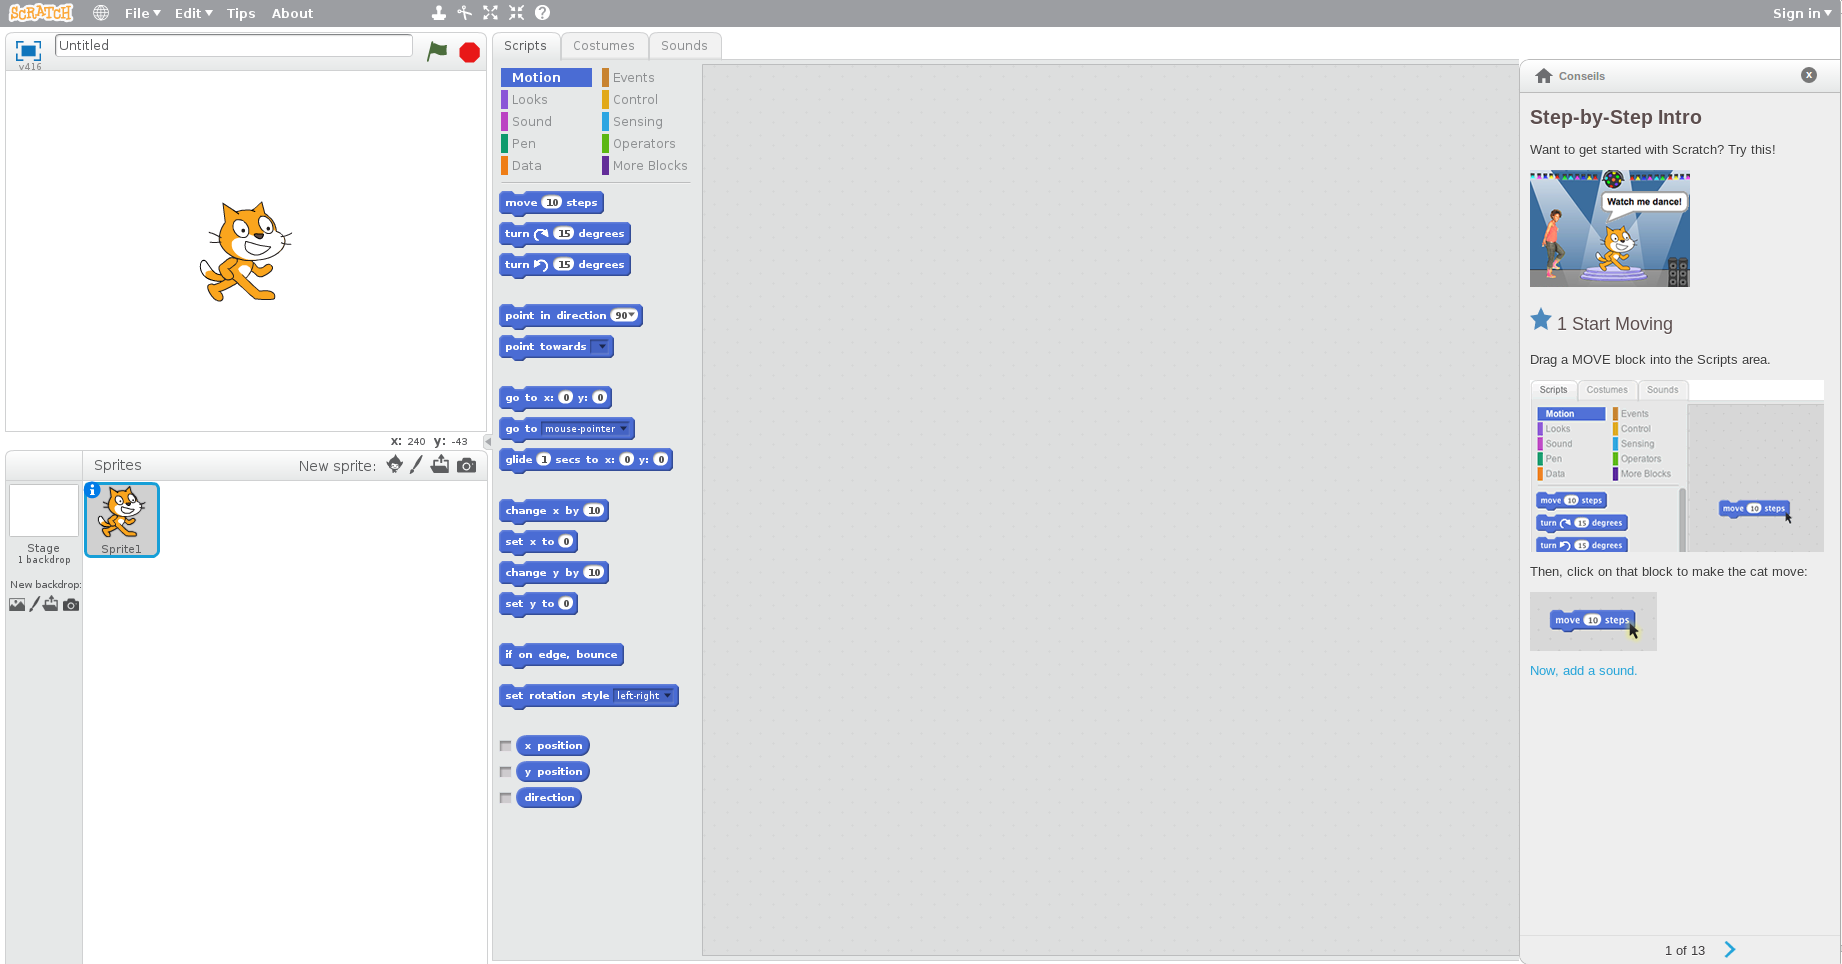
\includegraphics[width=\textwidth]{content/5-related_work/images/scratch-printscreen}
    \caption{Interface de Scratch}
    \label{fig:scratch-printscreen}
  \end{center}
\end{figure}

\subsection{Snap!}

\begin{figure}[!ht]
  \begin{center}
    
\includegraphics[scale=0.07]{content/5-related_work/images/snap}
    \caption{Logo de Snap!}
    \label{fig:snap}
  \end{center}
\end{figure}

Snap! \cite{snap} est un langage de programmation de "glisser-déposer" de \glspl{bloc}. C'est une ré-implémentation et une extension du langage Scratch du MIT. Il a été pensé et conçu pour être orienté web. Il est donc implémenté en JavaScript.\\

Ce langage est né en 2011 et a été créé par Jens Mönig, docteur de l'université de Berkeley. Il se distingue de son père Scratch par l'ajout de :
\begin{enumerate}
\item fonctions et procédures de première classe. Une entité dite de première classe est une entité qui supporte toutes les opérations disponibles sur d'autres entités. Un exemple est passer une fonction en paramètre ; %TODO glossaire premiere classe
\item listes de première classe. Un exemple est une liste de liste ;
\item \gls{sprite} de première classe. Un exemple est la composition de \gls{sprite}, par exemple personnage est représenté par un \gls{sprite} mais ses bras sont des sous-\glspl{sprite} qui peuvent soit se déplacer avec l'ensemble du corps soit de manière indépendante.
\end{enumerate}

\subsection{Python}

\begin{figure}[!ht]
  \begin{center}
    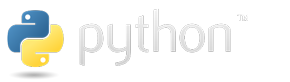
\includegraphics[scale=0.4]{content/5-related_work/images/python}
    \caption{Logo de Python}
    \label{fig:python}
  \end{center}
\end{figure}

Python \cite{python} est un langage de programmation qu'il ne faut plus présenter. Il a beaucoup d'avantages dont celui d'avoir une syntaxe légère et d'être facile à prendre en main. Une grande communauté et beaucoup de bibliothèques, dont la fameuse \texttt{turtle}, en fait un excellent langage pour démarrer dans la programmation.

Cependant, devoir apprendre un langage de programmation et la logique informatique en même temps complique la tâche. De plus, lorsqu'on commence un nouveau langage de programmation, il faut également apprendre ses bonnes pratiques de codage. %TODO retravailler pour être neutre

C'est donc un langage qui ne convient pas aux trop jeunes ni à ceux qui ne sont pas vraiment investis dans l'apprentissage de la programmation.
